\chapter{快速入门}\label{chapt:tour}

本章内容包括:

\begin{itemize}

\item 第一个Elixir程序
\item 使用交互式Elixir(iex)
\item 数据类型
\item 模式匹配
\item 列表与递归
\item 模块与函数
\item 管道(\texttt{|>})运算符
\item Erlang互操作性
\end{itemize}

我认为,与其深入每个语言特性,不如通过一系列示例来呈现它们。对于Java或Ruby程序员来说可能陌生的概念,我会进行更多的阐述。对于某些概念,您可能可以从您已知的任何语言中找到相似之处。这些示例会逐渐变得更有趣,几乎展示了理解本书中Elixir代码所需的所有内容。

\section{设置环境}

Elixir在所有主流编辑器上都得到了很好的支持,比如Vim、Emacs、Spacemacs、Atom、IntelliJ和VisualStudio。例如,专门为Emacs/Spacemacs与Elixir集成开发的Alchemist\pagenote{https://github.com/tonini/alchemist.el},提供了极佳的开发体验。它具有诸如文档查找、智能代码补全、与\texttt{iex}和\texttt{mix}的集成等众多有用的功能。与其他编辑器集成相比,它是支持最广泛、功能最丰富的。

准备好你的终端和编辑器,因为快速入门之旅现在就开始。

\section{第一步}

让我们从简单的开始。由于我曾经的殖民统治者(我来自新加坡),我对英尺、英寸及其亲戚们的度量单位不太熟悉。我们将编写一个长度转换器来解决这个问题。

以下是我们如何在Elixir中定义长度转换器的方法。输入以下内容到你最喜欢的文本编辑器中,并将文件保存为\texttt{length\_converter.ex}。

\begin{code}{Elixir中的长度转换程序}
\begin{minted}[linenos]{elixir}
defmodule MeterToFootConverter do
  def convert(m) do
    m * 3.28084
  end
end
\end{minted}
\label{lst:length_converter}
\end{code}

\texttt{defmodule} 定义一个新模块(即\texttt{MeterToFootConverter}),而\texttt{def} 定义一个新函数(即\texttt{convert})。

\subsection{在交互式Elixir中运行Elixir程序}

交互式Elixir,或简称\texttt{iex},相当于Ruby中的\texttt{irb} 或NodeJS中的\texttt{node}。在你的终端中,使用文件名作为参数启动\texttt{iex}。

\begin{code}{运行长度转换程序(\texttt{iex})}
\centering
\begin{minted}[linenos]{elixir}
% iex length_converter.ex
Erlang/OTP 26 [erts-14.2.1] [source] [64-bit] [smp:8:8] [ds:8:8:10] [async-threads:1] [jit] [dtrace]

Interactive Elixir (1.16.1) - press Ctrl+C to exit (type h() ENTER for help)
iex(1)>
\end{minted}
\label{lst:2-2}
\end{code}

世界上最高的男人的记录是2.72米。那是多少英尺?让我们找出答案:

\begin{code}{}
\begin{minted}[linenos]{elixir}
iex(1) > MeterToFootConverter.convert(2.72)
\end{minted}
% \label{lst:id}
\end{code}

结果是

\begin{code}{}
\begin{minted}[linenos]{elixir}
8.9238848
\end{minted}
% \label{lst:id}
\end{code}

\subsection{停止Elixir程序}

有几种方法可以停止Elixir程序,或者如果你想退出iex。第一种方法是输入\texttt{Ctrl + C}。第一次这样做时,你会看到:

\begin{code}{在iex中停止运行的Elixir程序}
\begin{minted}[linenos]{bash}
BREAK: (a)bort (A)bort with dump (c)ontinue (p)roc info (i)nfo
       (l)oaded (v)ersion (k)ill (D)b-tables (d)istribution
\end{minted}
\label{lst:stop_elixir_program}
\end{code}

你可以选择 \texttt{a)} 输入 \texttt{a}来中止,或者再次输入\texttt{Ctrl + C}。
另一种选择是使用\texttt{System.halt},虽然我个人更喜欢\texttt{Ctrl + C}。

\subsection{获取帮助}

由于\texttt{iex}是与Elixir交互的主要工具,因此学习更多关于它的信息是很有价值的。特别是,\texttt{iex}有一个非常棒的内置文档系统。再次启动\texttt{iex}。假设你想了解\texttt{Dict} 模块。你可以在\texttt{iex} 中输入\texttt{h Dict},输出将类似于图\ref{fig:2_3}。

\begin{figure}[!ht]
    \centering
    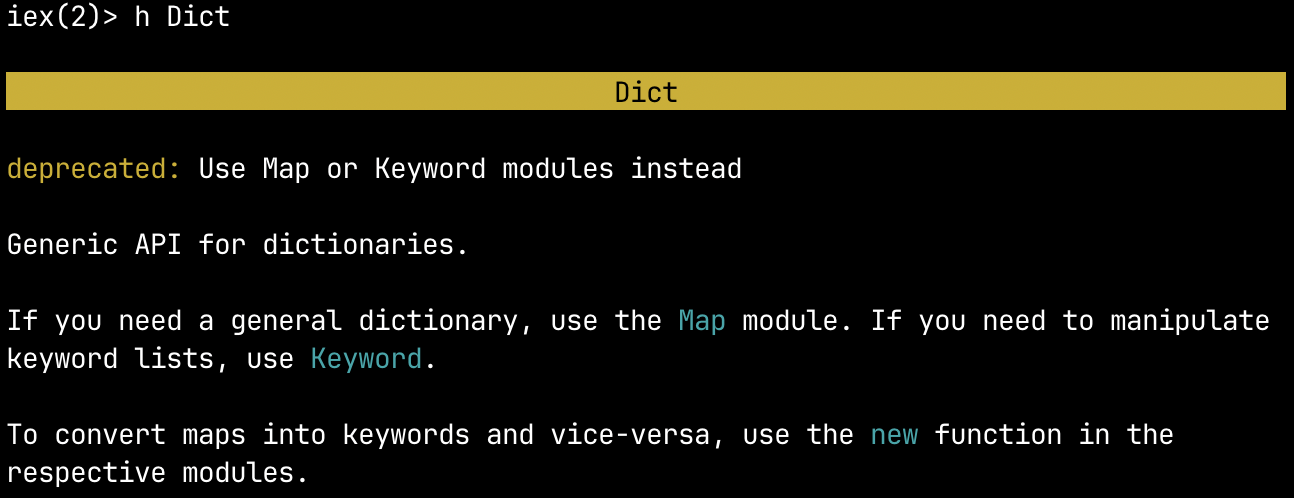
\includegraphics[width=0.8\linewidth]{2_3.png}
    \caption{在iex中显示的Dict模块文档}
    \label{fig:2_3}
\end{figure}


\texttt{Dict} 有哪些可用的函数?输入\texttt{Dict.}(重要的是后面的点\texttt{.}!),然后按你的\texttt{<Tab>} 键。你将看到\texttt{Dict} 模块中可用的函数列表,如图\ref{fig:2_4}所示。

\begin{figure}[!ht]
    \centering
    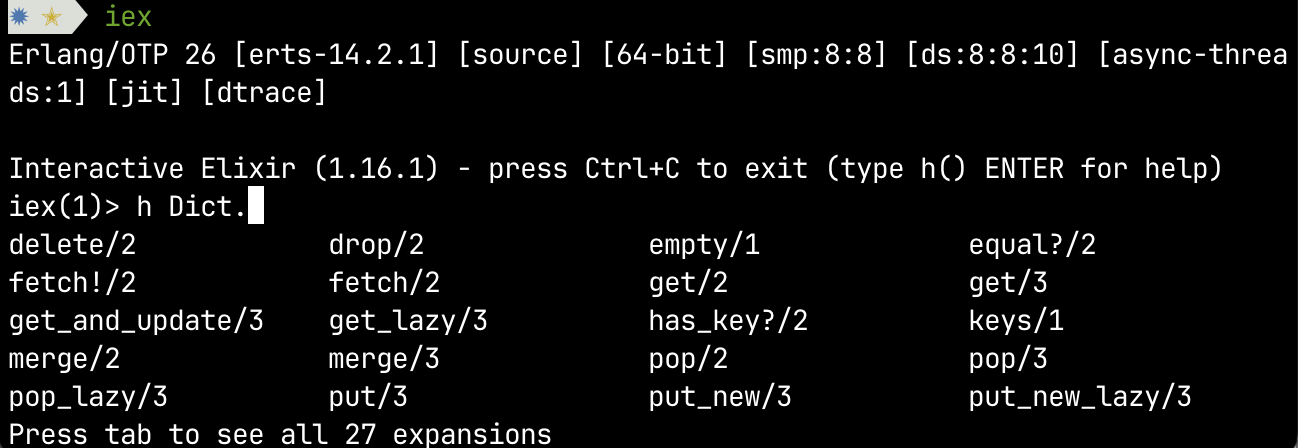
\includegraphics[width=0.8\linewidth]{2_4.png}
    \caption{\texttt{Dict} 模块中可用的函数列表}
    \label{fig:2_4}
\end{figure}


现在,假设你想了解更多关于 \texttt{put/3}函数。我稍后会解释 \texttt{/3}是什么意思。现在,它只意味着这个版本的 \texttt{put}接受3个参数。在 \texttt{iex} 中,输入\texttt{h Dict.put/3}。输出看起来像图\ref{fig:2_5}:

\begin{figure}[!ht]
    \centering
    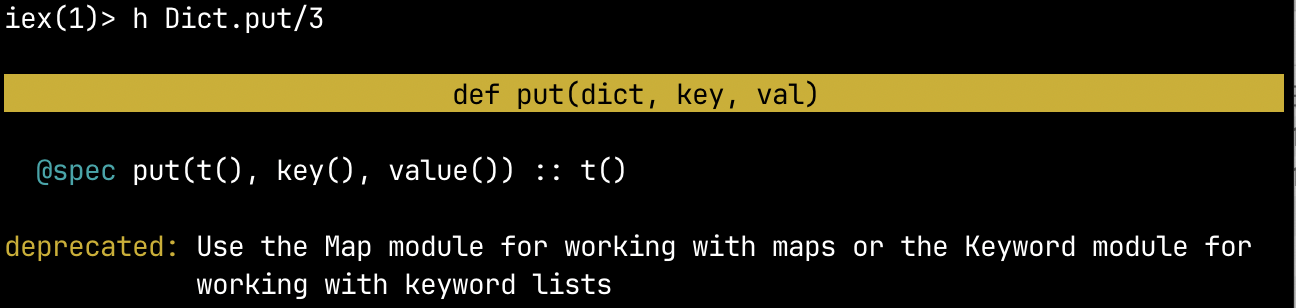
\includegraphics[width=0.8\linewidth]{2_5.png}
    \caption{\texttt{Dict.put/3} 的文档}
    \label{fig:2_5}
\end{figure}


相当整洁,对吧?更好的是,文档还有美观的语法高亮。

\begin{quote}
\textbf{注意}:因为本书成书较早,有许多内容已经过时。例如,你会注意到\texttt{h Dict}的输出中显示了deprecated的字样,表明该模块已被弃用。这是因为在Elixir 1.11中,\texttt{Dict}模块已被弃用。在Elixir1.11中,你应该使用\texttt{Map}模块。
\end{quote}

\section{数据类型}

在本书中,我们将使用以下常见数据类型:

\begin{itemize}

\item  模块(Modules)
\item  函数(Functions)
\item  数字(Numbers)
\item  字符串(Strings)
\item  原子(Atoms)
\item  元组(Tuples)
\item  映射(Maps)
\end{itemize}

\subsection{模块、函数和函数子句}

模块是Elixir用于将函数组合在一起的方式。模块的例子包括\texttt{List}、\texttt{String},当然还有\texttt{MeterToFootConverter}。使用\texttt{defmodule}创建模块。同样,使用\texttt{def}创建函数。


\subsubsection{模块}

让我们编写另一个函数,将米转换为\emph{英寸}。根据我们当前的实现,我们需要做一些更改。首先,我们的模块名太具体了。让我们将其更改为更通用的名称: \texttt{length\_converter.ex}。我们如何添加一个将米转换为英寸的函数?这是一种\emph{可能的}方法:


\begin{code}{\texttt{defmodules}可以嵌套}
\begin{minted}[linenos]{elixir}
defmodule MeterToLengthConverter do
  defmodule Feet do
    def convert(m) do
      m * 3.28084
    end
  end

  defmodule Inch do
    def convert(m) do
      m * 39.3701
    end
  end
end
\end{minted}
\label{lst:defmodules_can_be_nested}
\end{code}

现在,您可以计算最高的男人的身高(以英寸为单位):

\begin{code}{使用点表示法(\texttt{iex})}
\begin{minted}[linenos]{elixir}
iex > MeterToLengthConverter.Inch.convert(2.72)
\end{minted}
\label{lst:use_dot_notation}
\end{code}

返回\texttt{107.08667200000001}。这个例子说明了模块可以嵌套。这里,模块\texttt{Feet}和\texttt{Inch}嵌套在\texttt{MeterToLengthConverter}内。要访问嵌套模块中的函数,使用\emph{点表示法}。通常,要在Elixir中调用函数,使用以下格式:

\begin{code}{扁平化模块层次结构(\texttt{iex})}
\begin{minted}[linenos]{elixir}
Module.function(arg1, arg2, ...)
\end{minted}
\label{lst:flatten_module_hierarchy}
\end{code}

在邮件列表中,这有时被称为``\textbf{MFA}''。它代表\textbf{模块(Module)}、\textbf{函数(Function)}和\textbf{参数(Arguments)}。记住这种格式,因为您将在本书中再次遇到它。

您还可以像这样扁平化模块层次结构:

\begin{code}{}\begin{minted}[linenos]{elixir}
# 1
defmodule MeterToLengthConverter.Feet do
  def convert(m) do
    m * 3.28084
  end
end

# 1
defmodule MeterToLengthConverter.Inch do
  def convert(m) do
    m * 39.3701
  end
end

# 1 您可以使用点表示法来指定嵌套层次结构
\end{minted}
\end{code}


您将以与代码\ref{lst:use_dot_notation} 完全相同的方式调用该函数。


\subsubsection{函数和函数子句}

编写长度转换器的更习惯的方式是使用函数子句。这是我们长度转换器的修订版本:

\begin{code}{函数子句版本的长度转换器}
\begin{minted}[linenos]{elixir}
defmodule MeterToLengthConverter do
  def convert(:feet, m) do
    m * 3.28084
  end

  def convert(:inch, m) do
    m * 39.3701
  end
end
\end{minted}
\label{lst:function_clause_version_of_length_converter}
\end{code}

定义一个函数相当直接。大多数函数都是这样写的:

\begin{code}{函数的例子}
\begin{minted}[linenos]{elixir}
def convert(:feet, m) do
  m * 3.28084
end
\end{minted}
\label{lst:function_example}
\end{code}

单行函数这样写:

\begin{code}{单行函数}
\begin{minted}[linenos]{elixir}
def convert(:feet, m), do: m * 3.28084
\end{minted}
\label{lst:single_line_function}
\end{code}

既然我们提到了,让我们再添加一个将\emph{米}转换为\emph{码}的函数,这次使用单行变体:

\begin{code}{\texttt{length\_converter}的单行函数变体}
\begin{minted}[linenos]{elixir}
defmodule MeterToLengthConverter do
  def convert(:feet, m), do: m * 3.28084
  def convert(:inch, m), do: m * 39.3701
  def convert(:yard, m), do: m * 1.09361
end
\end{minted}
\label{lst:length_converter_single_line_function_variant}
\end{code}

函数按其\emph{元数}(它接受的参数数量)来引用。因此,我们将上述函数称为\texttt{convert/2}。\texttt{convert/2}是\emph{命名函数}的一个例子。Elixir还有\emph{匿名函数}的概念。这是一个匿名函数的常见例子:

\begin{code}{第二个参数是一个匿名函数(\texttt{iex})}
\begin{minted}[linenos]{elixir}
iex > Enum.map([1, 2, 3], fn x -> x * x end)
\end{minted}
\label{lst:second_argument_is_an_anonymous_function}
\end{code}

给出\texttt{[1, 4, 9]}

我们可以定义具有相同名称的多个函数,就像我们的示例中那样。需要注意的重要一点是它们\emph{必须}被分组在一起。因此,下面是一个错误示范:

\begin{code}{始终将相似的函数子句分组在一起}
\begin{minted}[linenos]{elixir}
defmodule MeterToLengthConverter do
  def convert(:feet, m), do: m * 3.28084
  def convert(:inch, m), do: m * 39.3701
  # 1
  def i_should_not_be_here, do: IO.puts("Oops")
  def convert(:yard, m), do: m * 1.09361
end

# 1 不要这样做!
\end{minted}
\label{lst:always_group_similar_function_clauses}
\end{code}


Elixir会相应地抱怨:
\begin{code}{当函数子句未分组在一起时,Elixir会抱怨}
\begin{minted}[linenos]{bash}
% iex length_converter.ex
    warning: clauses with the same name and arity (number of arguments) should be grouped together, "def convert/2" was previously defined (length_converter.ex:2)
    │
  5 │   def convert(:yard, m), do: m * 1.09361
    │       ~
    │
    └─ length_converter.ex:5:7
\end{minted}
\label{lst:elixir_complains_when_function_clauses_are_not_grouped_together}
\end{code}

另一个重要的事情:顺序很重要。每个函数子句都是自上而下匹配的。这意味着一旦Elixir找到一个兼容的函数子句匹配,它就会停止搜索并执行该函数。对于我们当前的长度转换器,移动函数子句不会影响任何事情。当我们稍后探讨递归时,您将开始理解函数子句顺序为何重要。

\subsection{数字(Numbers)}

在 Elixir 中,数字的运作方式和传统编程语言中的类似。

\begin{code}{操作整数、十六进制数和浮点数}
\begin{minted}[linenos]{elixir}
iex(1) > 1 + 0x2F / 3.0
16.666666666666664
\end{minted}
\label{lst:operating_on_integers_hexadecimal_numbers_and_floats}
\end{code}

\begin{code}{除法和余数函数}
\begin{minted}[linenos]{elixir}
iex(1) > div(10, 3)
3

iex(2) > rem(10, 3)
1
\end{minted}
\label{lst:dif_and_rem_functions}
\end{code}

\subsection{字符串(Strings)}

Elixir中的字符串有两种形态。表面上看,字符串看起来很标准。这里有一个展示字符串插值的例子:

\begin{code}{Elixir 支持字符串插值}
\begin{minted}[linenos]{elixir}
iex(1) > "字符串是 #{:great}!"
\end{minted}
\label{lst:elixir_supports_string_interpolation}
\end{code}

将给出:

\begin{code}{对字符串的操作}
\begin{minted}[linenos]{elixir}
"字符串是 great!"
\end{minted}
% \caption{Listing Caption}
% \label{lst:id}
\end{code}

我们还可以对字符串执行各种操作:

\begin{code}{}\begin{minted}[linenos]{elixir}
iex(2) > "字符串是 #{:great}!" |> String.upcase() |> String.reverse()
\end{minted}
% \label{lst:operating_on_strings}
\end{code}

这将返回:

\begin{code}{字符串是二进制数据}
\begin{minted}[linenos]{elixir}
"!TAERG 是串符字"
\end{minted}
% \caption{Listing Caption}
% \label{lst:id}
\end{code}


\subsubsection{字符串是二进制数据(Binaries)。}

如何测试一个字符串?没有 \texttt{is\_string/1}函数可用。这是因为在 Elixir中,字符串是一种\textbf{二进制数据}。二进制数据只是一个字节序列。

\begin{code}{}\begin{minted}[linenos]{elixir}
iex(3) > "字符串是二进制数据" |> is_binary
\end{minted}
% \label{lst:strings_are_binaries}
\end{code}

返回\texttt{true}。

展示字符串的二进制表示的一种方式是使用二进制串联运算符\texttt{<>}来附加一个空字节,\texttt{<<0>>}:

\begin{code}{展示字符串的二进制表示}
\begin{minted}[linenos]{elixir}
iex(4) > "ohai" <> <<0>>
\end{minted}
\label{lst:showing_the_binary_representation_of_a_string}
\end{code}

返回 \mintinline{elixir}|<<111, 104, 97, 105, 0>>|

每个数字代表一个字符:

\begin{code}{字符串不是字符列表}
\begin{minted}[linenos]{elixir}
iex(5) > ?o
111
iex(6) > ?h
104
iex(7) > ?a
97
iex(8) > ?i
105
\end{minted}
% \caption{Listing Caption}
% \label{lst:id}
\end{code}

为了进一步确信二进制表示与原字符串等价:

\begin{code}{}\begin{minted}[linenos]{elixir}
iex(44) > IO.puts(<<111, 104, 97, 105>>)
\end{minted}
% \caption{Listing Caption}
% \label{lst:id}
\end{code}

将给你原始字符串:

\begin{code}{}\begin{minted}[linenos]{elixir}
ohai
:ok
\end{minted}
% \caption{Listing Caption}
% \label{lst:id}
\end{code}


\subsubsection{字符串不是字符列表(Char lists)}

顾名思义,字符列表是字符的列表。它与字符串是完全不同的数据类型,这可能会有些混淆。虽然字符串总是用双引号括起来,字符列表则用单引号括起来。

\begin{code}{}\begin{minted}[linenos]{elixir}
iex(9) > ~c"ohai" == "ohai"
\end{minted}
% \label{lst:strings_are_not_char_lists}
\end{code}

将给出 \texttt{false}。你通常不会使用字符列表,至少在Elixir 中不会。然而,当与某些 Erlang库交互时,你可能需要这样做。例如,在后面的示例中,Erlang 的 http客户端(httpc)接受字符列表作为 URL:\mintinline{elixir}|:httpc.request 'http://www.elixir-lang.org'|
如果我们传入字符串(二进制数据)会发生什么呢?试试看:

\begin{code}{:httpc.request/1 期望 URL 类型为字符列表}
\begin{minted}[linenos]{elixir}
iex(51)> :httpc.request "http://www.elixir-lang.org"
** (ArgumentError) 
:erlang.tl("http://www.elixir-lang.org")
(inets) inets_regexp.erl:80: :inets_regexp.first_match/3
(inets) inets_regexp.erl:68: :inets_regexp.first_match/2
(inets) http_uri.erl:186: :http_uri.split_uri/5
(inets) http_uri.erl:136: :http_uri.parse_scheme/2
(inets) http_uri.e

l:88: :http_uri.parse/2
(inets) httpc.erl:162: :httpc.request/5
\end{minted}
\label{lst:httpc_request_1_expects_the_url_to_be_a_char_list}
\end{code}


我们将在本章后面进一步讨论调用 Erlang 库的内容,但当你处理某些 Erlang库时,这是你需要记住的事情。

 \subsection{原子 (Atoms)}

原子在Elixir中作为常量存在,有点类似于Ruby中的符号。原子总是以冒号开始。创建原子有两种不同的方式:\texttt{:hello\_atom}和\texttt{:"Hello Atom"}都是有效的原子。需要注意的是,原子和字符串并不相同,因为原子和字符串是完全不同的数据类型。

\begin{code}{原子不是字符串}
\begin{minted}[linenos]{elixir}
iex > :hello_atom == "hello_atom"
false
\end{minted}
\label{lst:atoms_are_not_strings}
\end{code}

单独来看,原子并不是非常有趣。然而,当我们将原子放入\emph{元组}中,并在\emph{模式匹配}的上下文中使用它们时,你就会开始理解原子的作用以及Elixir如何利用原子编写声明性代码。我们将在后面几节中讨论模式匹配。现在,让我们转向元组。

 \subsection{元组 (Tuples)}

一个元组可以包含不同类型的数据。例如,一个HTTP客户端可能以元组的形式返回一个成功的请求:
\mintinline{elixir}|{200, "http://www.elixir-lang.org"}|
一个失败的请求可能看起来像这样:
\mintinline{elixir}|{404, "http://www.php-is-awesome.org"}|

元组使用基于零的访问方式,就像在大多数编程语言中访问数组元素一样。因此,如果你想要获取请求结果的URL,你需要传入\texttt{1}给\texttt{elem/2}:

\begin{code}{访问元组中的第二个元素}
\begin{minted}[linenos]{elixir}
iex > elem({404, "http://www.php-is-awesome.org"}, 1)
\end{minted}
\label{lst:accessing_the_second_element_of_a_tuple}
\end{code}

这将返回 \texttt{http://www.php-is-awesome.org}。
你可以使用\texttt{put\_elem/3}来更新一个元组:

\begin{code}{更新一个元组}
\begin{minted}[linenos]{elixir}
iex > put_elem({404, "http://www.php-is-awesome.org"}, 0, 503)
\end{minted}
\label{lst:update_a_tuple}
\end{code}

返回 \mintinline{elixir}|{503, "http://www.php-is-awesome.org"}|

\subsection{映射 (Maps)}

映射本质上是键值对,类似于哈希或字典,具体取决于你所使用的语言。所有映射操作都通过\texttt{Map}模块暴露。

使用映射相当直接,但需要注意一个小问题。看看你是否能在例子中发现它。让我们从一个空映射开始:

\begin{code}{创建一个新的映射}
\begin{minted}[linenos]{elixir}
iex > programmers = Map.new()
%{}
\end{minted}
\label{lst:create_a_new_map}
\end{code}

让我们向映射中添加一些聪明的人:

\begin{code}{向映射中添加元素}
\begin{minted}[linenos]{elixir}
iex > programmers = Map.put(programmers, :joe, "Erlang")
%{joe: "Erlang"}
iex > programmers = Map.put(programmers, :matz, "Ruby")
%{joe: "Erlang", matz: "Ruby"}
iex > programmers = Map.put(programmers, :rich, "Clojure")
%{joe: "Erlang", matz: "Ruby", rich: "Clojure"}
\end{minted}
\label{lst:add_elements_to_a_map}
\end{code}

\textbf{一个非常重要的旁白:不可变性 (Immutability)}

注意到\texttt{programmers}是\texttt{Map.put/3}的一个参数,并且\emph{重新绑定}到\texttt{programmers}上。为什么会这样?

\begin{code}{为额外检查添加守卫}
\begin{minted}[linenos]{elixir}
iex > Map.put(programmers, :rasmus, "PHP")
%{joe: "Erlang", matz: "Ruby", rasmus: "PHP", rich: "Clojure"}
\end{minted}
\label{lst:adding_guards_for_extra_checks}
\end{code}

返回值包含了新的条目。让我们检查一下\texttt{programmers}的内容:

\begin{code}{}\begin{minted}[linenos]{elixir}
iex > programmers
%{joe: "Erlang", matz: "Ruby", rich: "Clojure"}
\end{minted}
% \caption{Listing Caption}
% \label{lst:id}
\end{code}

这个属性被称为\textbf{不可变性}。

Elixir中的\textbf{所有}数据结构都是不可变的,这意味着你无法对其进行任何修改。你所做的任何修改\textbf{总是}保留原始结构\textbf{不变}。相反,返回一个修改过的副本。因此,为了捕获结果,你可以将其重新绑定到同一个变量名,或者将值绑定到另一个变量上。

\section{守卫(Guards)}

让我们再次看看
\texttt{length\_converter.ex}。假设我想确保参数始终是数字。我们可以通过添加守卫子句来修改程序:

\begin{code}{}\begin{minted}[linenos]{elixir}
defmodule MeterToLengthConverter do
  def convert(:feet, m) when is_number(m), do: m * 3.28084 #1
  def convert(:inch, m) when is_number(m), do: m * 39.3701 #1
  def convert(:yard, m) when is_number(m), do: m * 1.09361 #1
end
\#1 在函数子句中添加守卫。
\end{minted}
% \label{lst:id}
\end{code}


所以现在,如果你尝试像\mintinline{elixir}|{MeterToLengthConverter.convert(:feet, "smelly")}|这样有趣的事情,没有任何函数子句会匹配。实际上,Elixir会抛出一个\texttt{FunctionClauseError}:

\begin{code}{尝试执行上述代码会导致 FunctionClauseError}
\begin{minted}[linenos]{elixir}
iex(1)> MeterToLengthConverter.convert (:feet, "smelly")
** (FunctionClauseError) no function clause matching in MeterToLengthConverter.convert/2

    The following arguments were given to MeterToLengthConverter.convert/2:

        # 1
        :feet

        # 2
        "smelly"

    length_converter.ex:2: MeterToLengthConverter.convert/2
    iex:1: (file)
\end{minted}
\label{lst:trying_to_execute_the_above_code_will_result_in_a_functionclauseerror}
\end{code}

负长度没有意义。让我们确保参数是非负的。我们可以通过添加另一个守卫表达式来实现这一点:

\begin{code}{我们可以在守卫中包含简单表达式}
\begin{minted}[linenos]{elixir}
defmodule MeterToLengthConverter do
  # 1
  def convert(:feet, m) when is_number(m) and m >= 0, do: m * 3.28084
  # 1
  def convert(:inch, m) when is_number(m) and m >= 0, do: m * 39.3701
  # 1
  def convert(:yard, m) when is_number(m) and m >= 0, do: m * 1.09361
end

# 1 检查 m 是否为非负数
\end{minted}
\label{lst:we_can_include_simple_expressions_in_guards}
\end{code}


除了\texttt{is\_number/1},当你需要区分不同的数据类型时,还有其他类似的函数会派上用场。要生成这个列表,启动\texttt{iex},然后输入 \texttt{is\_}后跟 \texttt{<Tab>} 键。

\begin{code}{在 iex 中使用自动补全来发现函数名称}
\begin{minted}[linenos]{elixir}
iex(1)> is_
is_atom/1         is_binary/1       is_bitstring/1    is_boolean/1
is_exception/1    is_exception/2    is_float/1        is_function/1
is_function/2     is_integer/1      is_list/1         is_map/1
is_map_key/2      is_nil/1          is_number/1       is_pid/1
is_port/1         is_reference/1    is_struct/1       is_struct/2
Press tab to see all 21 expansions
\end{minted}
\label{lst:using_autocompletion_in_iex_to_discover_function_names}
\end{code}

\texttt{is\_*} 函数应该是非常直观的,除了\texttt{is\_port/1} 和\texttt{is\_reference/1}。我们在这本书中不会使用端口。稍后我们会遇到引用,你将看到它们在为消息赋予唯一身份时是如何有用的。

守卫子句在消除条件语句方面特别有用,正如你所猜测的,它们在确保你的参数是正确类型时也很有用。

\section{模式匹配}

模式匹配是函数式编程语言中最强大的功能之一,而Elixir也不例外。事实上,模式匹配是我最喜欢的Elixir功能之一。一旦你看到模式匹配能做什么,你就会开始渴望在不支持它们的语言中使用它们。

Elixir使用等号(\texttt{=})来执行模式匹配。与大多数语言不同,Elixir不仅使用\texttt{=}操作符进行变量赋值。事实上,\texttt{=}被称为\emph{匹配操作符}。从现在开始,当你看到一个\texttt{=}时,不要想它是等于,而是匹配。我们究竟在匹配什么呢?简而言之,模式匹配用于匹配值和数据结构。在接下来的示例中,你将了解为什么\texttt{=}被称为匹配操作符。更重要的是,你将学会爱上模式匹配,作为一种生成优美代码的强大工具。首先,让我们学习规则:


\subsection{\texttt{=}用于赋值}

匹配操作符的第一个规则是:变量赋值仅在变量位于表达式的\emph{左}侧时发生。

\begin{code}{变量赋值仅在变量位于左侧时发生}
\begin{minted}[linenos]{elixir}
iex > programmers = Map.put(programmers, :jose, "Elixir")
\end{minted}
\label{lst:variable_assignment_only_happens_when_the_variable_is_on_the_left}
\end{code}

将产生:
\texttt{\%\{joe: "Erlang", jose: "Elixir", matz: "Ruby", rich: "Clojure"\}}

这里,我们将\texttt{Map.put/2}的结果赋值给了\texttt{programmers}。预期中,\texttt{programmers}包含:

\begin{code}{}
\begin{minted}[linenos]{elixir}
iex > programmers
%{joe: "Erlang", jose: "Elixir", matz: "Ruby", rich: "Clojure"}
\end{minted}
% \label{lst:id}
\end{code}


\subsection{\texttt{=}也用于匹配}

现在事情变得稍微有趣一些。让我们交换一下我们之前的表达式顺序:

\begin{code}{匹配Map(在左侧)与\texttt{programmers}}
\begin{minted}[linenos]{elixir}
iex > %{joe: "Erlang", jose: "Elixir", matz: "Ruby", rich: "Clojure"} = programmers
%{joe: "Erlang", jose: "Elixir", matz: "Ruby", rich: "Clojure"}
\end{minted}
\label{lst:match_a_map_against_programmers}
\end{code}

在这里,我们调换了顺序。注意这\emph{不是}一个赋值。相反,发生了一次\emph{成功的模式匹配},因为左侧的内容和\texttt{programmers}是相同的。让我们看一个\emph{不成功}的模式匹配:

\begin{code}{一个不成功的模式匹配}
\begin{minted}[linenos]{elixir}
iex> %{tolkien: "Elvish"} = programmers
** (MatchError) no match of right hand side value: %{joe: "Erlang", jose: "Elixir", matz: "Ruby", rich: "Clojure"}
\end{minted}
\label{lst:an_unsuccessful_pattern_match}
\end{code}
当一个不成功的匹配发生时,会抛出一个\texttt{MatchError}。

\subsection{解构}
接下来我们来看看解构,因为我们需要用到它来执行一些模式匹配的酷炫技巧。
解构是模式匹配发挥作用的地方。\emph{the Common Lisp Language}\pagenote{http://www.cs.cmu.edu/Groups/AI/html/cltl/clm/node252.html}中对解构的定义是:

\emph{解构允许你将一组变量绑定到相应的值集合,这可以在任何你能将一个值绑定到单个变量的地方进行。}

用代码来解释的话:

\begin{code}{将左侧的变量绑定到右侧的值}
\begin{minted}[linenos]{elixir}
iex > %{joe: a, jose: b, matz: c, rich: d} =
  %{joe: "Erlang", jose: "Elixir", matz: "Ruby", rich: "Clojure"}
\end{minted}
\label{lst:bind_the_variables_on_the_left_to_the_values_on_the_right}
\end{code}

下面是每个变量的内容:

\begin{code}{仅匹配部分模式}
\begin{minted}[linenos]{elixir}
iex > a
"Erlang"
iex > b
"Elixir"
iex > c
"Ruby"
iex > d
"Clojure"
\end{minted}
% \caption{Listing Caption}
% \label{lst:id}
\end{code}

这里,我们将一组\emph{变量}(\texttt{a}、\texttt{b}、\texttt{c}和 \texttt{d})绑定到相应的一组\emph{值}(\texttt{Erlang}、\texttt{Elixir}、\texttt{ Ruby }和\texttt{Clojure})。如果你只对提取部分信息感兴趣怎么办?没问题,因为你可以进行模式匹配,而不需要指定整个模式:

\begin{code}{}\begin{minted}[linenos]{elixir}
iex > %{jose: most_awesome_language} = programmers
%{joe: "Erlang", jose: "Elixir", matz: "Ruby", rich: "Clojure"}
iex > most_awesome_language
"Elixir"
\end{minted}
% \label{lst:matching_only_part_of_a_pattern}
\end{code}

这在你只对提取少量信息感兴趣时非常方便。这里是Elixir程序中经常使用的另一种有用技术。注意这两个表达式的返回值:

\begin{code}{成功的提取返回\mintinline{elixir}|{:ok, value}|}
\begin{minted}[linenos]{elixir}
iex > Map.fetch(programmers, :rich)
{:ok, "Clojure"}
\end{minted}
\label{lst:successful_fetch_returns_ok_value}
\end{code}

\begin{code}{不成功的提取返回\texttt{:error}}
\begin{minted}[linenos]{elixir}
iex > Map.fetch(programmers, :rasmus)
:error
\end{minted}
\label{lst:unsuccessful_fetch_returns_error}
\end{code}

注意,当找到键时返回一个包含原子 \texttt{:ok}和值的元组,否则返回 \texttt{:error}原子。这里你将看到元组和原子是如何有用的,以及我们如何利用模式匹配来利用这些返回值。通过利用正确路径和异常路径的返回值,我们可以这样表达自己:

\begin{code}{处理正确路径和错误路径}
\begin{minted}[linenos]{elixir}
iex(14)> case Map.fetch(programmers, :rich) do #1
...(14)> {:ok, language} -> IO.puts "#{language} is a legit language."
...(14)> :error -> IO.puts "No idea what language this is."
...(14)> end
\end{minted}
\label{lst:handling_the_happy_path_and_the_error_path}
\end{code}

这将返回

\begin{code}{读取文件}
\begin{minted}[linenos]{elixir}
Clojure is a legit language.
:ok
\end{minted}
% \caption{Listing Caption}
% \label{lst:id}
\end{code}


\begin{example}{读取文件}
\end{example}

这种技术非常适用于在程序中声明前提条件。我的意思是什么?以读取文件为例。如果你的大部分逻辑依赖于文件的\emph{可读性},那么尽早知道文件读取出现错误的情况是有意义的。知道发生了什么类型的错误也会有所帮助。以下是\texttt{File.read/1} 文档的片段:

\begin{figure}[!ht]
    \centering
    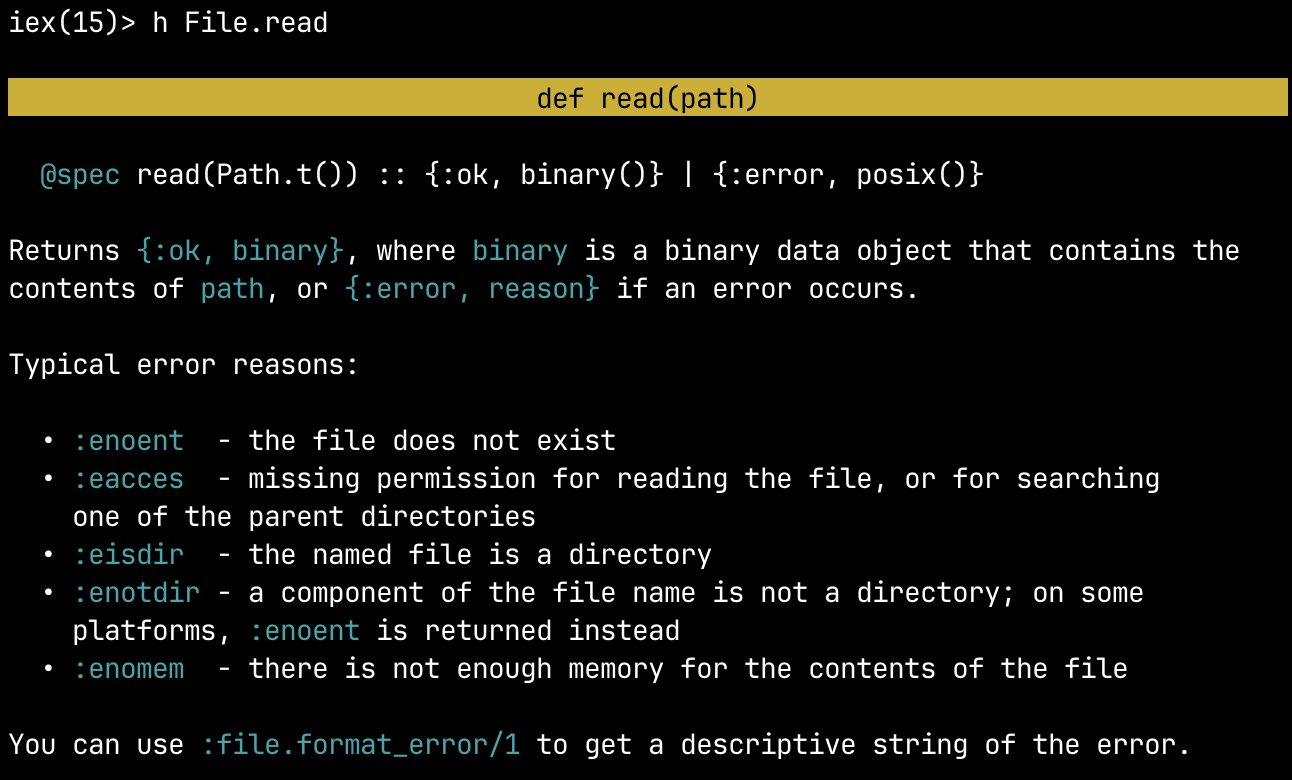
\includegraphics[width=0.8\linewidth]{2_6.png}
    \caption{File.read/1 的文档}
    \label{fig:2_6}
\end{figure}

你会如何编写文件读取部分?更重要的是,从上述文档中我们能学到什么?

\begin{enumerate}
\def\labelenumi{\arabic{enumi}.}

\item
  对于成功的读取,\texttt{File.read/1} 返回一个
  \mintinline{elixir}|{:ok, binary}| 元组。注意
  \texttt{binary} 是读取文件的全部内容。
\item
  否则,将返回 \mintinline{elixir}|{:error, reason}| 元组。变量
  \texttt{reasob}包含错误原因,这是一个原子,如
  \texttt{:enoent} 或
  \texttt{:eacces}。
\end{enumerate}


\begin{code}{}\begin{minted}[linenos]{elixir}
case File.read("KISS - Beth.mp3") do
  {:ok, binary} ->
    IO.puts("KISS rocks!")

  {:error, reason} ->
    IO.puts("No Rock N Roll for anyone today because of #{reason}.")
end
\end{minted}
% \label{lst:reading_a_file}
\end{code}


\begin{example}{井字棋盘}

以下是使用元组的井字棋应用程序的一个示例。在这个例子中,我们有一个\texttt{check\_board/1}函数,它检查井字棋的棋盘配置。棋盘是使用元组表示的。注意我们如何使用元组``绘制''棋盘,以及代码是多么易于理解:

\begin{code}{}% \captionof{listing}{井字棋}
\begin{minted}[linenos]{elixir}
def check_board(board) do
  case board do
    {:x, :x, :x, _, _, _, _, _, _} -> :x_win
    {_, _, _, :x, :x, :x, _, _, _} -> :x_win
    {_, _, _, _, _, _, :x, :x, :x} -> :x_win
    {:x, _, _, :x, _, _, :x, _, _} -> :x_win
    {_, :x, _, _, :x, _, _, :x, _} -> :x_win
    {_, _, :x, _, _, :x, _, _, :x} -> :x_win
    {:x, _, _, _, :x, _, _, _, :x} -> :x_win
    {_, _, :x, _, :x, _, :x, _, _} -> :x_win
    # Player O board patterns omitted ...

    {a, b, c, d, e, f, g, h, i} when a and b and c and d and e and f and g and h and i -> :draw
    _ -> :in_progress
  end
end
\end{minted}
% \label{lst:tictactoe}
\end{code}

`\texttt{\_}' 是 ``不关心'' 或 ``匹配一切''运算符。在本书中你将看到很多这样的例子。在下一节中,我们将看到更多模式匹配的例子,其中我们将讨论\emph{列表}。
\end{example}

\begin{example}{解析MP3文件}
\end{example}

Elixir非常适合解析二进制数据。在这个例子中,我们将从MP3文件中提取元数据。这也是一个很好的练习,以加强你之前学到的一些概念。在解析任何二进制之前,你必须知道文件布局(layout)。我们感兴趣的信息,\emph{ID3标签},位于mp3二进制的\emph{最后128字节}:

\begin{figure}[!ht]
    \centering
    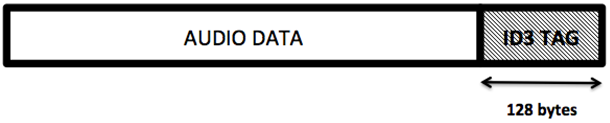
\includegraphics[width=0.8\linewidth]{2_7.png}
    \caption{ID3标签位于MP3二进制的最后128字节。}
    \label{fig:2_7}
\end{figure}

这意味着我们必须以某种方式忽略音频数据部分,只关注ID3标签。下图显示了ID3标签的布局:

\begin{figure}[!ht]
    \centering
    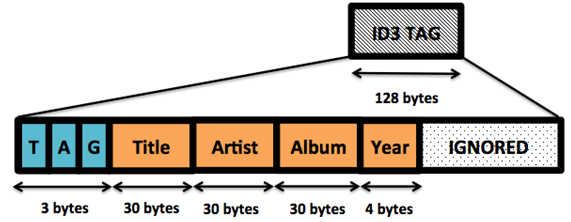
\includegraphics[width=0.8\linewidth]{2_8.png}
    \caption{ID3标签的布局}
    \label{fig:2_8}
\end{figure}

ID3标签的前三个字节称为头部,包含三个字符:``T'',``A''和``G''。接下来的30个字节包含\emph{标题(title)}。然后是30个字节的\emph{艺术家(artist)},接着是另外30个字节的\emph{专辑(album)}。接下来的4个字节是\emph{年份(year)}(例如:``2'',``0'',``1'',``4'')。试想你会如何在其他编程语言中实现这一点。这是Elixir版本的实现,请将此文件保存为\texttt{id3.ex}。

\begin{code}{}
\begin{minted}[linenos]{elixir}
defmodule ID3Parser do
  def parse(file_name) do
    case File.read(file_name) do #1
      {:ok, mp3} -> #2
        mp3_byte_size = byte_size(mp3) – 128 #4
        << _ :: binary-size(mp3_byte_size), id3_tag :: binary >> = mp3 #5 使用模式匹配从MP3二进制数据中捕获ID3标签的字节。
        << "TAG", title   :: binary-size(30),
          artist  :: binary-size(30),
          album   :: binary-size(30),
          year    :: binary-size(4),
          _rest   :: binary >>       = id3_tag #6
        IO.puts "#{artist} - #{title} (#{album}, #{year})"
      _ -> #3
        IO.puts "Couldn't open #{file_name}"
    end
  end
end

#1 读取MP3二进制数据。
#2 成功读取文件返回一个匹配此模式的元组。
#3 文件读取失败则与其他任何内容匹配。
#4 计算MP3音频部分的字节大小。
#5 使用模式匹配从MP3二进制数据中捕获ID3标签的字节。
#6 使用模式匹配从ID3标签中捕获各种ID3字段。
\end{minted}
% \label{lst:id}
\end{code}



程序运行示例:

\begin{code}{}
\begin{minted}[linenos]{elixir}
% iex id3.ex
iex(1)> ID3Parser.parse "sample.mp3"
\end{minted}
% \label{lst:id}
\end{code}

程序运行结果示例:

\begin{code}{}
\begin{minted}[linenos]{elixir}
Lana Del Rey - Ultraviolence (Ultraviolence, 2014)
:ok
\end{minted}
% \label{lst:id}
\end{code}

让我们来回顾一下程序的运行过程。首先,程序读取MP3的二进制数据。正常情况下会返回一个匹配\mintinline{elixir}|{:ok, mp3}|的元组,其中\texttt{mp3}包含文件的二进制内容。否则,通用的\texttt{\_}操作符将匹配文件读取失败的情况。

由于我们只关注ID3标签,因此需要找到一种方法来``跳过''前面的部分。我们首先计算二进制音频部分的\emph{字节大小}。现在我们有了这个信息,就可以告诉Elixir如何解构二进制数据。我们通过在左边声明一个模式,并在右边使用mp3变量来进行模式匹配。请记住,变量赋值在左边,否则尝试进行模式匹配。

\begin{figure}[!ht]
    \centering
    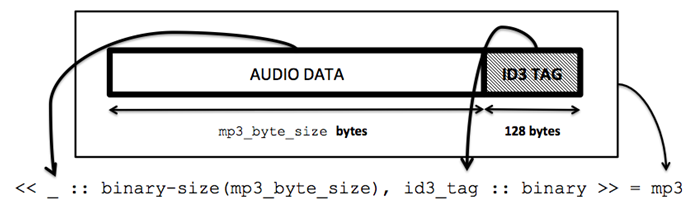
\includegraphics[width=0.8\linewidth]{2_9.png}
    \caption{二进制数据的解构方式}
    \label{fig:2_9}
\end{figure}

你可能认出了\texttt{<< >>}。它用于表示一个二进制数据。然后我们声明我们对音频部分不感兴趣。我们如何做到这一点呢?我们通过指定之前计算出的二进制大小来实现。剩下的就是ID3标签,被捕获到\texttt{id3\_tag}变量中。现在我们可以自由地从ID3标签中提取信息了!

为了做到这一点,我们进行了另一个模式匹配,左边声明了模式,右边是\texttt{id3\_tag}。通过声明适当数量的字节,标题、艺术家和其他信息被捕获到相应的变量中。

\begin{figure}[!ht]
    \centering
    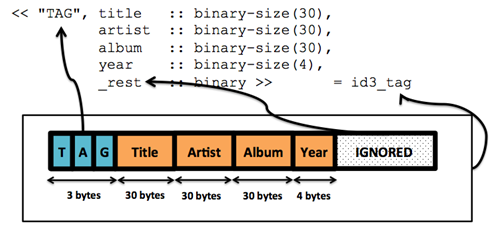
\includegraphics[width=0.8\linewidth]{2_10.png}
    \caption{解构ID3二进制数据}
    \label{fig:2_10}
\end{figure}

\section{列表}

列表是 Elixir
中的另一种数据类型。列表有许多有趣的用途,因此值得单独讨论。列表在某种程度上类似于\emph{链表}\pagenote{http://en.wikipedia.org/wiki/Linked\_list},因为随机访问基本上是一个
O(n) 线性操作。下面是列表的定义:

\begin{quote}
\textbf{一个非空列表由头部和尾部组成。尾部也是一个列表。}
\end{quote}

请注意上述定义的递归性质。转换成代码就是:

\begin{code}{}
\begin{minted}[linenos]{elixir}
iex > [1, 2, 3] == [1 | [2 | [3 | []]]]
true
\end{minted}
% \label{lst:id}
\end{code}

一个图示可能更能说明这一点:

\begin{figure}[!ht]
    \centering
    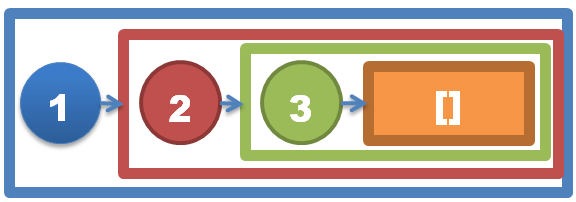
\includegraphics[width=0.8\linewidth]{2_11.png}
    \caption{[1,2,3]的图示表示}
    \label{fig:2_11}
\end{figure}


让我们从最外层的盒子开始理解这幅图。这表明列表的头部是1,随后是列表的尾部。这个尾部,又是另一个列表。这次,这个列表的头部是2,随后是尾部,这个尾部(再次)是另一个列表。

最终,这个列表(从第三个封闭盒子)由一个头部 3和一个尾部组成。这个尾部是一个空列表。实际上,\emph{任何列表的最后一个元素的尾部总是一个空列表}。递归函数利用这一事实来确定列表何时结束。

您还可以使用模式匹配运算符来证明两边确实是同一回事:

\begin{code}{左侧和右侧是等价的}
\begin{minted}[linenos]{elixir}
iex > [1, 2, 3] = [1 | [2 | [3 | []]]]
[1, 2, 3]
\end{minted}
\label{lst:left_and_right_are_equivalent}
\end{code}

由于没有\texttt{MatchError}发生,我们可以确定这两种表示列表的方法是等价的。当然,您不会在日常代码中输入\texttt{[1|[2|[3|[]]]]}。这只是为了强调列表是一种递归数据结构。

我还没有解释`\texttt{|}'是什么。'\texttt{|}'运算符通常被称为\emph{cons}运算符\pagenote{\texttt{construct}的缩写. 参考\url{http://en.wikipedia.org/wiki/Cons}获得更多信息.}。应用于列表时,它用于分隔头部和尾部。也就是说,列表被\emph{解构}了。这是模式匹配的又一个实例。

\begin{code}{使用 cons 运算符解构列表}
\begin{minted}[linenos]{elixir}
iex > [head | tail] = [1, 2, 3]
[1, 2, 3]
\end{minted}
\label{lst:use_the_cons_operator_to_destructure_a_list}
\end{code}

让我们检查 head 和 tail 的内容:

\begin{code}{}
\begin{minted}[linenos]{elixir}
iex > head
1
# A``[2, 3]`
iex > tail
# A 这也是一个列表
\end{minted}
% \label{lst:id}
\end{code}

注意\texttt{tail}也是一个列表,这符合定义。您还可以使用cons 运算符向列表的开头\emph{添加}(或追加):

\begin{code}{使用 cons 运算符向列表中追加}
\begin{minted}[linenos]{elixir}
iex(1) > list = [1, 2, 3]
[1, 2, 3]
iex(2) > [0 | list]
[0, 1, 2, 3]
\end{minted}
\label{lst:use_the_cons_operator_to_append_to_a_list}
\end{code}

我们还可以使用\texttt{++}运算符来连接列表:

\begin{code}{使用 ++ 运算符连接列表}
\begin{minted}[linenos]{elixir}
iex(3) > [0] ++ [1, 2, 3]
[0, 1, 2, 3]
\end{minted}
\label{lst:use_the_++_operator_to_concatenate_lists}
\end{code}

那么单个元素的列表呢?如果您理解了之前的列表图示,那么这将是小菜一碟。

\begin{code}{单元素列表的尾部匹配为空列表}
\begin{minted}[linenos]{elixir}
iex(22) > [head | tail] = [:lonely]
[:lonely]
iex(23) > head
:lonely
iex(24) > tail
[]
\end{minted}
\label{lst:single_element_list_tail_matches_an_empty_list}
\end{code}

这里我们有一个包含单个原子的列表。现在注意我们的\texttt{tail}是一个空列表。起初这可能看起来有些奇怪,但如果您仔细思考,它符合定义。正是这种定义使我们能够用列表和递归做一些有趣的事情,我们接下来会进行探索。


\begin{example}{展平列表}
\end{example}

现在您了解了列表的工作原理,让我们来构建我们自己的\texttt{flatten/1}。\texttt{flatten/1}接受一个可能嵌套的列表,并返回一个展平的版本。展平列表特别有用,尤其是当列表用于表示树\pagenote{http://en.wikipedia.org/wiki/Tree\_\%28data\_structure\%29\#Representations}数据结构时。因此,展平树会返回树中包含的所有元素。让我们看一个例子:

\begin{code}{}
\begin{minted}[linenos]{elixir}
List.flatten([1, [:two], ["three", []]])
\end{minted}
% \label{lst:id}
\end{code}

将返回\texttt{[1, :two, "three"]}。这是\texttt{flatten/1} 的一种可能实现:

\begin{code}{展平列表的可能实现}
\begin{minted}[linenos]{elixir}
defmodule MyList do
  def flatten([]), do: [] #1
  def flatten([ head | tail ]) do  #2
    flatten(head) ++ flatten(tail) #2
  end
  def flatten(head), do: [ head ]  end #3

#1 基本情况,一个空列表
#2 非空列表,有多于 1 个元素
#3 单元素列表
\end{minted}
\label{lst:possible_implementation_of_flattening_a_list}
\end{code}


花点时间消化这段代码,因为它不仅仅是表面看起来那样。需要考虑3种情况:

我们从基本情况(或者如果您上过一些计算机科学课程的话,退化情况)开始------ 空列表:

1. 如果我们得到一个空列表,我们只需返回一个空列表。 

2. 对于非空列表,我们使用 cons运算符将其分解为\texttt{head}和\texttt{tail}。然后我们递归地调用\texttt{flatten/1}处理\texttt{head}和\texttt{tail}。接下来,使用\texttt{++}运算符将结果连接起来。注意\texttt{head}也可能是一个嵌套列表。例如,\texttt{[[1], 2]}意味着\texttt{head}是\texttt{[1]}。

如果我们得到一个非列表参数,我们将其转换成一个列表。现在,考虑(最好在纸上跟踪)对像\texttt{[[1], 2]}
这样的列表的处理。让我们跟踪执行过程:

1. 第一个函数子句 \#1 不匹配。 

2. 第二个函数子句 \#2匹配。在这种情况下,我们对列表进行模式匹配,\texttt{head}是\texttt{[1]},而\texttt{tail}是\texttt{2}。现在,\texttt{flatten([1])}和\texttt{flatten(2)}被递归调用。

3. 处理\texttt{flatten([1])}。它同样不匹配第一个子句\#1。第二个子句 \#2匹配。~\texttt{head}~是\texttt{1},而\texttt{tail}是\texttt{[]}。

4. 现在调用\texttt{flatten(1)},第三个函数子句 \#3匹配,返回\texttt{[1]}。\texttt{flatten[])}匹配第一个子句,返回\texttt{[]}。之前对\texttt{flatten(2)}的调用(见第2步)返回\texttt{[2]}。\texttt{[1] ++ [] ++ [2]}生成了我们的展平列表。

不要灰心,如果你第一次没有完全理解。就像大多数事情一样,多一些练习会有很大的帮助。此外,在接下来的章节中,你将看到许多例子。

\subsection{函数子句(Function Clauses)的排序}

我之前提到过,函数子句(Function Clauses)的\emph{顺序}很重要。这是一个完美的例子来解释为什么:

\begin{code}{函数子句(Function Clauses)的顺序很重要}
\begin{minted}[linenos]{elixir}
defmodule MyList do
  def flatten([head | tail]) do
    flatten(head) ++ flatten(tail)
  end

  def flatten(head), do: [head]

  # 1 这行永远不会运行!
  def flatten([]), do: []
end
\end{minted}
\label{lst:the_order_of_function_clauses_is_important}
\end{code}

我们将基本情况设为了最后一个子句。想一想,当我们尝试\texttt{MyList.flatten([])}时会发生什么?我们期望得到\texttt{[]},但实际上我们得到了\texttt{[[]]}。如果你仔细思考一下,你会意识到\#1从未被执行。原因是第二个函数子句会匹配\texttt{[]},因此第三个函数子句将被忽略。

让我们真正运行一下这个程序:


\begin{code}{Elixir 会有帮助地警告未匹配的子句}
\begin{minted}[linenos]{elixir}
% iex length_converter.ex
warning: this clause cannot match because a previous clause at line 7 always matches
\end{minted}
\label{lst:elixir_will_helpfully_warn_about_unmatched_clauses}
\end{code}

Elixir在背后默默支持我们!像这样的警告值得注意,因为它们可以节省你数小时的调试头痛。而未匹配的条款可能意味着无效代码,或者在更糟糕的情况下,是一个无限循环。

\section{管道运算符\texttt{|>}}

现在,我想介绍编程语言史上最有用的运算符之一 -\texttt{|>} \pagenote{\texttt{|>} 操作符收到了F\#的启发.}。
这个运算符将左边表达式的结果作为右边函数调用的第一个参数。这是我最近写的一个Elixir程序中的代码片段。如果没有管道运算符,我会这样写它:

\begin{code}{没有 \texttt{|>}运算符(或者,大多数语言的做法)}
\begin{minted}[linenos]{elixir}
defmodule URLWorker do
  def start(url) do
    do_request(HTTPoison.get(url))
  end

  # ...
end
\end{minted}
\label{lst:without_the_pipe_operator_or_the_way_most_languages_do_it}
\end{code}

\texttt{HTTPoison} 是一个 HTTP 客户端。它接收一个\texttt{url} 并返回 HTML 页面。然后将页面传递给\texttt{do\_request}函数进行一些解析。注意,在这个版本中,你必须寻找最内层的括号来定位\texttt{url},然后在你脑子里追踪连续的函数调用向外移动。

我向你展示带有管道运算符的版本:

\begin{code}{使用 \texttt{|>} 运算符}
\begin{minted}[linenos]{elixir}
defmodule URLWorker do
  def start(url) do
    result = url |> HTTPoison.get() |> do_request
  end

  # ...
end
\end{minted}
\label{lst:use_pipe_operator}
\end{code}

很清晰对吧?许多例子将广泛使用 \texttt{|>}。你越多使用\texttt{|>},就越会开始看到\emph{数据正在从一种形式转换}到另一种,就像装配线一样。事实上,一旦你经常使用它,当你在其他语言中编程时,你会开始想念它。


\begin{example}{按文件名过滤目录中的文件}
\end{example}

假设我有一个装满电子书的目录,这个目录可能嵌套有文件夹。我想只获取 EPUB的文件名。例如,我只想要文件名以 \texttt{*.epub}
结尾且包含 ``Java'' 的书籍。这是我的做法:

\begin{code}{过滤包含 ``Java'' 的 epub}
\begin{minted}[linenos]{elixir}
# 1
"/Users/Ben/Books"
# 2
|> Path.join("**/*.epub")
# 3
|> Path.wildcard()
# 4
|> Enum.filter(fn fname ->
  String.contains?(Path.basename(fname), "Java")
end)
\end{minted}
\label{lst:filter_epubs_containing_java}
\end{code}

\#1 是目录的字符串表示。在 \#2中,我们构造了一个带通配符的路径。此外,我们指定我们只对 EPUB感兴趣。这个结果传递给\#3。通配符函数读取路径,并返回匹配的文件名列表。这反过来又传递到 \#4中的过滤函数,只选择包含 ``Java''的文件名。阅读如此明确和显而易见地描述其步骤的代码是非常好的。

一个示例输出看起来像:
\begin{minted}[linenos]{bash}
["/Users/Ben/Books/Java/Java_Concurrency_In_Practice.epub",
 "/Users/Ben/Books/Javascript/JavaScript Patterns.epub",
 "/Users/Ben/Books/Javascript/Functional_JavaScript.epub",
 "/Users/Ben/Books/Ruby/Using_JRuby_Bringing_Ruby_to_Java.epub"]
\end{minted}

 \section{Erlang与Elixir互操作性}

由于Elixir和Erlang共享相同的字节码,因此在性能方面调用Erlang代码不会有任何影响。更重要的是,这意味着您可以自由地使用任何Erlang库与您的Elixir代码一起使用。

\subsection{从Elixir调用Erlang函数}

唯一的注意点是\emph{如何}调用代码。例如,您可以像这样在Erlang中生成一个随机数:

\begin{code}{在Erlang中生成随机数}
\begin{minted}[linenos]{erlang}
1> random:uniform(123)
55
\end{minted}
\label{lst:generate_a_random_number_in_erlang}
\end{code}

这个函数是Erlang标准发行版的一部分。我可以在Elixir中用一些语法调整调用相同的Erlang函数:


\begin{code}{将 \texttt{random:uniform().}翻译为Elixir}
\begin{minted}[linenos]{elixir}
iex > :random.uniform(123)
55
\end{minted}
\label{lst:use_the_random_uniform_function_in_elixir}
\end{code}

注意两个代码中冒号和点的位置。这就是全部!在Elixir中使用原生Erlang函数时有一个小注意点。您无法从\texttt{iex}访问Erlang函数的文档:

\begin{code}{在iex中无法获得Erlang文档}
\begin{minted}[linenos]{elixir}
iex(3)> h :random
:random 是一个Erlang模块,因此它没有Elixir风格的文档
\end{minted}
\label{lst:cannot_get_erlang_docs_in_iex}
\end{code}

调用Erlang函数在Elixir中没有相应实现的标准库时非常有用。如果您比较Erlang和Elixir的标准库,可能会得出Erlang的库功能更加丰富的结论。但如果您仔细想想,Elixir实际上免费获得了一切!


\subsubsection{在Elixir中调用Erlang的HTTP客户端}

通常,如果我发现Elixir缺少我想要的某个功能,我会首先检查是否有Erlang标准库函数可以使用,然后才搜索第三方库。例如,我曾想在Elixir中构建一个网络爬虫。构建网络爬虫的第一步之一就是能够下载网页。这需要一个HTTP客户端。Elixir没有内置的HTTP客户端------它不需要,因为Erlang有一个,恰当地命名为\texttt{httpc}\pagenote{http://erlang.org/doc/man/httpc.html\#request-1}。

假设我想下载某个编程语言的网页。我查阅了Erlang文档\pagenote{骗你的,在现实中我可能会首先访问StackOverflow},找到了我需要的内容:

\begin{figure}[!ht]
    \centering
    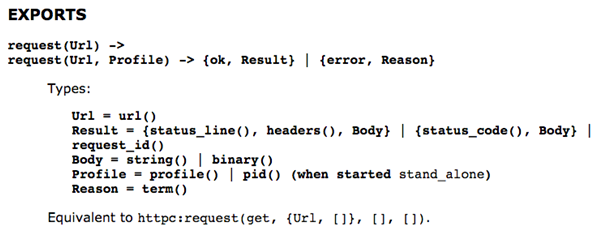
\includegraphics[width=0.8\linewidth]{2_6a.png}
    \caption{Erlang文档中的httpc:request/1}
    \label{fig:2_6a}
\end{figure}

首先,我需要启动\texttt{inets}应用程序(文档中有说明),然后进行实际的请求:


\begin{code}{使用Erlang的httpc库下载网页}
\begin{minted}[linenos]{elixir}
iex(1)> :inets.start
:ok
iex(2)> {:ok, {status, headers, body}} = :httpc.request 'http://www.elixir-lang.org'
{:ok,
 {{'HTTP/1.1', 200, 'OK'},
  [{'cache-control', 'max-age=600'}, {'date', 'Tue, 28 Oct 2014 16:17:24 GMT'},
   {'accept-ranges', 'bytes'}, {'server', 'GitHub.com'},
   {'vary', 'Accept-Encoding'}, {'content-length', '17251'},
   {'content-type', 'text/html; charset=utf-8'},
   {'expires', 'Tue, 28 Oct 2014 16:27:24 GMT'},
   {'last-modified', 'Tue, 21 Oct 2014 23:38:22 GMT'}],
  [60, 33, 68, 79, 67, 84, 89, 80, 69, 32, 104, 116, 109, 108, 62, 10, 60, 104,
   116, 109

, 108, 32, 120, 109, 108, 110, 115, 61, 34, 104, 116, 116, 112, 58, 47, 47, 119, 119, 119, 46, 119, 51, 46, 111, 114, 103, 47, 49, 57, 57, ...]}}
\end{minted}
\label{lst:downloading_a_web_page_with_erlangs_httpc_library}
\end{code}


\subsubsection{还有一件事\ldots\ldots{}}

Erlang还有一个非常整洁的GUI前端,名为\emph{Observer},让您能够检查Erlang虚拟机等内容。调用它很简单:

\begin{code}{调用Observer,一个内置的Erlang工具}
\begin{minted}[linenos]{elixir}
iex(1) > :observer.start()
\end{minted}
\label{lst:use_erlang_observer}
\end{code}

由于您当前没有运行任何计算密集型进程,因此现在不会看到太多动作。图\ref{fig:2_7a}供您预览:

\begin{figure}[!ht]
    \centering
    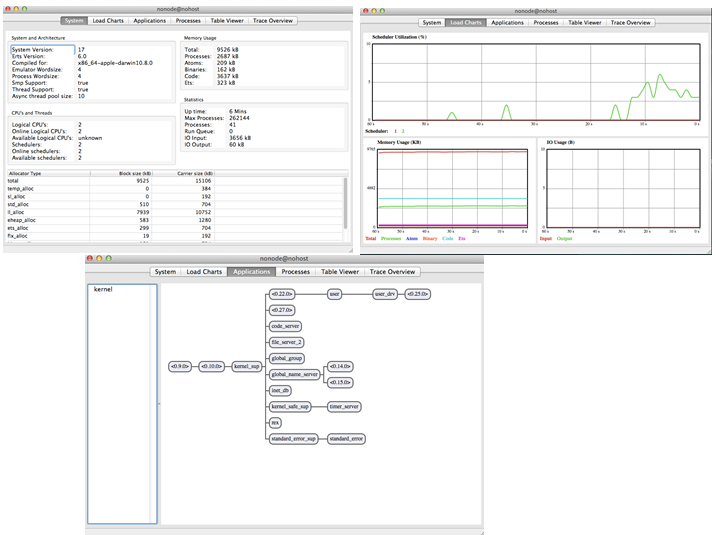
\includegraphics[width=0.8\linewidth]{2_7a.png}
    \caption{Observer的截图}
    \label{fig:2_7a}
\end{figure}

Observer在查看VM承受的负载、监督树的布局(您将在后面的章节学习到这一点)以及查看Erlang提供的内置数据库中存储的数据方面非常有用。

 \section{练习}

这是一个相当长的章节。现在是时候确保你理解了章节中的所有内容。

\begin{enumerate}
\def\labelenumi{\arabic{enumi}.}

\item 实现 \texttt{sum/1}函数。这个函数应该接收一个数字列表,并返回该列表的总和。
\item 探索 \texttt{Enum} 模块。
\item 将 \texttt{[1,[[2],3]]} 转换为\texttt{[9, 4, 1]},分别使用和不使用管道操作符。
\item 将 Erlang 中的\texttt{crypto:md5("Tales from the Crypt").} 翻译为
  Elixir。
\item 探索官方的 Elixir入门指南
	  \pagenote{http://elixir-lang.org/getting\_started/1.html}。
\item
  看看一个 IPV4 数据包。尝试编写一个解析器。
\end{enumerate}

\section{总结}

这结束了我们的快速旅程。如果你坚持到了这里,请给自己一个赞。如果你还没有理解所有内容,不用担心。许多概念会在途中变得清晰,一旦你看到它们的应用,许多编程结构会变得显而易见。作为一个快速回顾,这里是我们刚刚学到的内容:

\begin{itemize}

\item  Elixir 的基本数据类型。
\item  守护子句(Guards),以及它们如何与函数子句很好地协作。
\item  模式匹配,以及它如何导致非常声明式的代码。我们还看了一些模式匹配的实际例子。
\item  列表,另一个基本的数据结构。我们还看到了列表在 Elixir  中如何内部表示,以及这如何促进递归。
\item  Elixir 和 Erlang 如何良好地协同工作。
\end{itemize}

在下一章中,我们将学习 Elixir 中并发的基本单位------进程。这是 Elixir与传统编程语言截然不同的特性之一。

\printnotes*